\documentclass[11pt]{article}
\usepackage[utf8]{inputenc}
\usepackage[T1]{fontenc}
\usepackage{geometry}
\usepackage{amsmath}
\usepackage{amsfonts}
\usepackage{amssymb}
\usepackage{graphicx}
% \usepackage{natbib}
\usepackage{url}
\usepackage{hyperref}
\usepackage{titlesec}
\usepackage{enumitem}
\usepackage{wrapfig}
\usepackage[backend=biber, style=numeric, sorting=none]{biblatex}
\addbibresource{ref.bib}

\usepackage{booktabs}
\usepackage{array}
\usepackage{caption}
\usepackage{subcaption}
\usepackage{lmodern}
\usepackage{microtype}
\usepackage{threeparttable}   % for threeparttable and tablenotes
\captionsetup{font=scriptsize, labelfont=bf, position=top, skip=3pt}
\setlength{\tabcolsep}{4pt}
\renewcommand{\arraystretch}{1.05}

% Page layout
\geometry{
    left=0.8in,
    right=0.6in,
    top=0.6in,
    bottom=0.8in
}
\newcommand{\ts}{\mathrm{TS}}
\newcommand{\jsd}{\mathrm{JSD}}
\newcommand{\tsw}{\mathrm{TS_{wild}}}
\newcommand{\inm}{\mathrm{Infl}}
\newcommand{\adj}{\mathrm{Adj}}
\newcommand{\K}[1]{{\color{red}[[\textbf{K: }#1]]}}
\newcommand{\E}[1]{{\color{blue}#1}}
\newcommand{\facin}{f(\mathrm{act/inh})}
\newcommand{\ewnum}{\mathrm{EW_{num}}}
\newcommand{\tsten}{\mathrm{Toggle Switch (10N,100E)}}
\newcommand{\tstwo}{\mathrm{Toggle Switch (10N,80E)}}
\newcommand{\tsfour}{\mathrm{Toggle Switch (10N,60E)}}
\newcommand{\tssix}{\mathrm{Toggle Switch (10N,40E)}}
\newcommand{\tseight}{\mathrm{Toggle Switch (10N,20E)}}
\newcommand{\emttwosix}{\mathrm{EMT (23N,89E)}}
\newcommand{\emtrac}{\mathrm{EMT (17N,62E)}}
\newcommand{\gonad}{\mathrm{Gonadal (18N,74E)}}
\newcommand{\siltwo}{\mathrm{Silviera (18N,37E)}}
\newcommand{\sil}{\mathrm{Silviera (16N,30E)}}
\newcommand{\sclc}{\mathrm{SCLC (33N,357E)}}
\newcommand{\tennode}{\mathrm{NRF2 + OVOL (8N,19E)}}
\newcommand{\twenode}{\mathrm{NRF2 + GRHL2 + OVOL (11N,28E)}}
\newcommand{\beginsupplement}{%
        \setcounter{table}{0}
        \renewcommand{\thetable}{S\arabic{table}}%
        \setcounter{figure}{0}
        \renewcommand{\thefigure}{S\arabic{figure}}%
        \setcounter{section}{0}
        \renewcommand{\thesection}{S\arabic{section}}%
     }

%%%%%%%%%%%%%%%%%%%%%%%%%%%%%%%%%%%%%%%%%%%%%%%%%%
\title{Regulatory stochasticity drives opposing phenotypic outcomes in cell-fate decision networks}

\author{Kishore Hari$^1$, Abhay Gupta$^2$, Lakshmi Malvadi$^3$, Prakash Kulkarni$^4$, Ravi Salgia$^4$, \\ Mohit Kumar Jolly$^3$, Herbert Levine$^1$}



\begin{document}


\maketitle
\begin{center}
    $^1$ Center for Theoretical Biological Physics \& Department of Physics, Northeastern University, Boston, USA\\
    $^2$ Indian Institute of Science Education and Research Mohali, Mohali, USA\\
    $^3$ Department of Bioengineering, Indian Institute of Science, Bengaluru, India \\
    $^4$ Department of Medical Oncology and Therapeutics Research, and Department of Systems Biology, City of Hope National Medical Center, Duarte, CA, USA \\
\end{center}

\begin{center}
    \textbf{Current address}: Abhay Gupta, Department of Biology, University of Virginia, Charlottesville, USA\\
\textbf{Current address}: Lakshmi Malvadi, Department of Physics, University of California Merced, Merced, USA
\end{center}
\begin{abstract}
Models of gene regulatory networks (GRNs) underlying cell-fate decision systems treat regulatory parameters as fixed quantities, although transcription-factor efficacy varies with molecular context. We asked how temporal fluctuations in interaction strength, rather than molecular abundance, alter phenotype occupancy in multistable regulatory networks. We applied three stochastic update rules to fold-change parameters—independent fluctuations anchored to their initial values, a bounded additive random walk, and a bounded multiplicative random walk—across RACIPE ensembles of mutually inhibitory circuits, and tested analogous perturbations in Boolean models of epithelial–mesenchymal plasticity and gonadal-fate determination. Anchored fluctuations largely preserved deterministic occupancies of network states. Additive fluctuations increased occupancy of all-high co-expression states, particularly in multistable regimes and when high expression was readily accessible; this effect extended to hybrid team-expression states in both biological networks. Multiplicative fluctuations biased inhibitory fold changes toward stronger repression and favored single-high states in a topology-dependent manner. Fixed-parameter controls sampled from the same noise-induced distributions did not fully reproduce the additive effect or the multiplicative effect in several circuits. A Boolean-limit analysis traced the additional additive bias to an asymmetry between unconditional derepression and conditional repression. Thus, temporally evolving regulatory parameters can redistribute phenotype occupancy in ways not predicted from static parameter ensembles, with outcomes jointly determined by fluctuation dynamics and network topology.
\end{abstract}


\begin{figure}
    \centering
    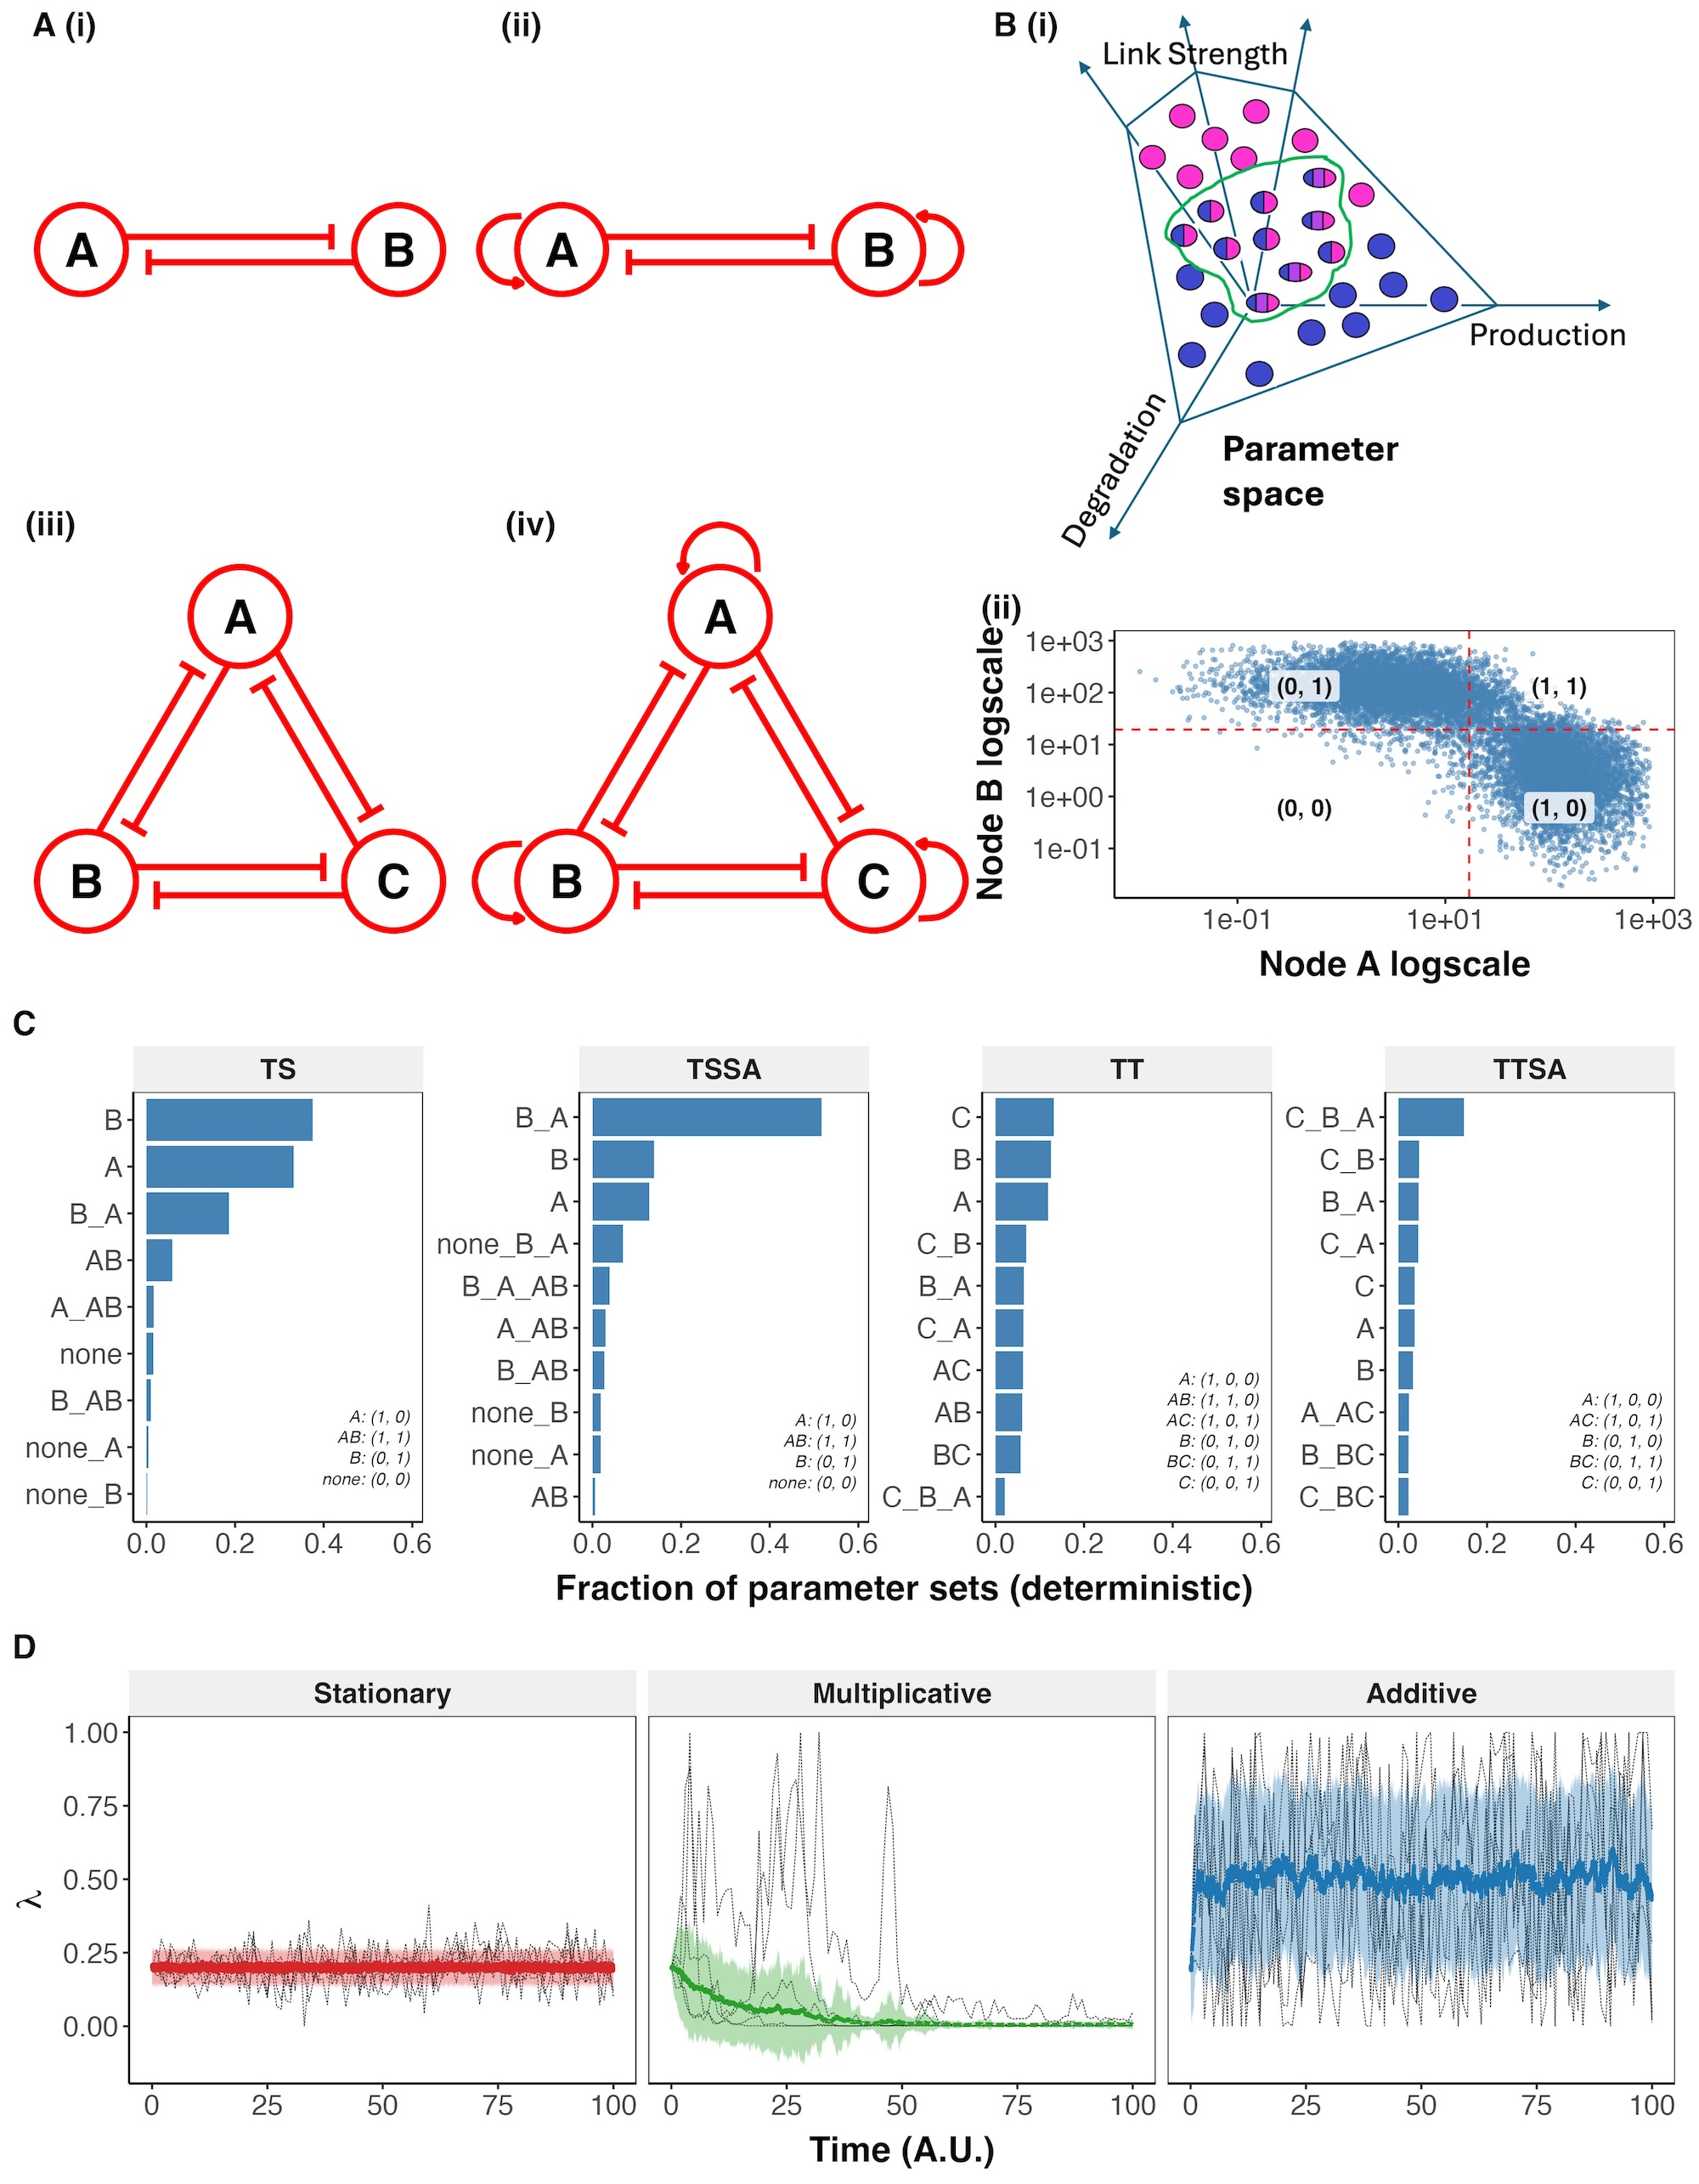
\includegraphics[width=0.8\linewidth]{Figs/Fig1.jpg}
    \caption{
    \textbf{RACIPE network topologies and the stochastic simulation framework.}. 
    \textbf{(A)} Network topology diagrams for the four base circuits used throughout this study: (i) TS (toggle switch), (ii) TSSA (toggle switch with self-activation), (iii) TT (toggle triad), (iv) TTSA (toggle triad with self-activation). Red circles denote nodes; bar-headed edges denote inhibitory interactions; curved arrows denote self-activation.
    \textbf{(B)} (i) Schematic of the RACIPE parameter-sampling framework: production, degradation, and interaction-strength parameters are randomly sampled within a bounded parameter space, generating an ensemble of models with varying dynamical behavior. (ii) Steady-state expression of node A vs. node B (log scale) across the RACIPE parameter ensemble for the TS network. Dashed red lines mark each gene's discretization threshold (mean of its expression in log scale across all steady states); quadrants are labeled with the corresponding discrete state, (A, B).
    \textbf{(C)} Frequency of the 10 most frequent discrete attractors found by RACIPE for each network (TS, TSSA, TT, TTSA), expressed as the fraction of parameter sets that map onto these attractors. States are represented in short-hand form, with the key given inside the plot. Compound labels (e.g.\ ``A\_B'') denote multistable parameter sets. Because TT and TTSA support many more distinct multistable combinations than TS/TSSA, the top-10 bars shown capture only part of the full ensemble: 100\%, 99.2\%, 77.5\%, and 46.2\% of all parameter sets for TS, TSSA, TT, and TTSA respectively (out of 9, 12, 97, and 119 total distinct attractor combinations found).
    \textbf{(D)} Simulated trajectories of the fold-change parameter $\lambda(t)$ under the three stochastic noise-update rules used in this study (Stationary, Multiplicative, Additive), shown for an inhibitory-edge-range parameter ($\lambda \in [0,1]$, $\lambda_0 = 0.2$). Thin black dashed lines show 5 representative individual trajectories (sampled once per time unit for legibility); the colored line and shaded ribbon show the mean $\pm$ SD across 100 simulated trajectories.}
    \label{fig:1}
\end{figure}

\begin{figure}
    \centering
    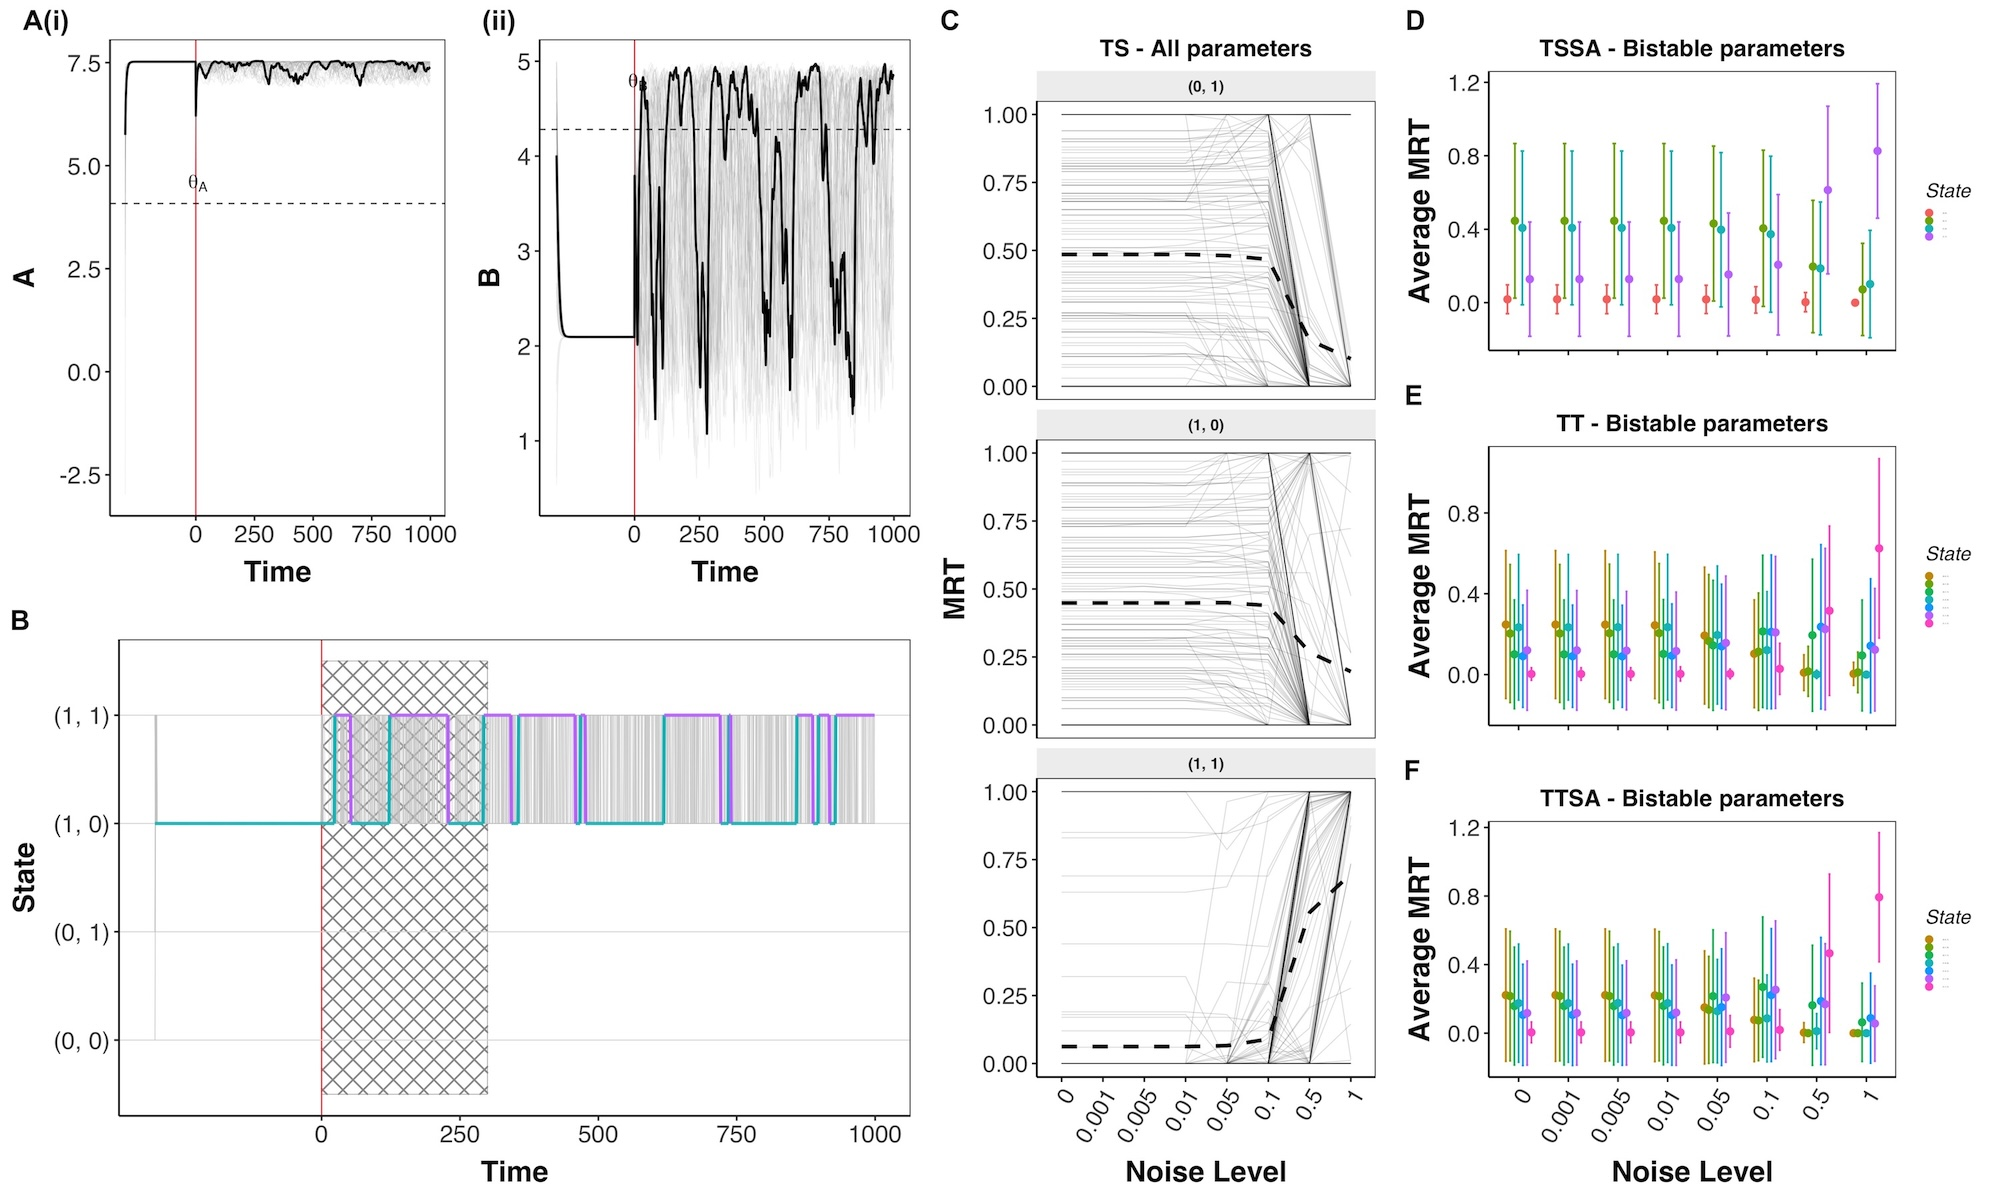
\includegraphics[width=\linewidth]{Figs/Fig2.jpg}
    \caption{\textbf{Effect of stationary noise on toggle switch and toggle triad networks}. 
    \textbf{(A)} Representative single-parameter trajectory for the TS network: (i) node A and (ii) node B expression over time (log$_2$), with the deterministic (noise-free) segment at negative time and the stochastic segment at positive time. Gray lines show all sampled initial conditions; the black line highlights one representative trajectory (the one whose switch count is closest to the population median); dashed horizontal line marks each node's discretization threshold $\theta$.
    \textbf{(B)} Discrete-state trace of the same parameter, colored by state for the highlighted trajectory (gray for all other initial conditions). Crosshatched region marks the discarded transient-dominated window of the stochastic segment. 
    \textbf{(C)} MRT of each state across noise levels. Each panel corresponds to the state indicated by its label. Grey lines show individual parameter-set trajectories; the black dashed line shows their mean. Darker or apparently solid grey segments result from the overlap of multiple trajectories and do not denote a separate category.
    \textbf{(D--F)} MRT vs.\ noise level for TSSA (D), TT (E), and TTSA (F) bistable parameter sets, colored by state (top 4 states shown for TSSA, top 7 for TT/TTSA), mean $\pm$ SD across parameter sets. 
}
    \label{fig:2}
\end{figure}

\begin{figure}
    \centering
    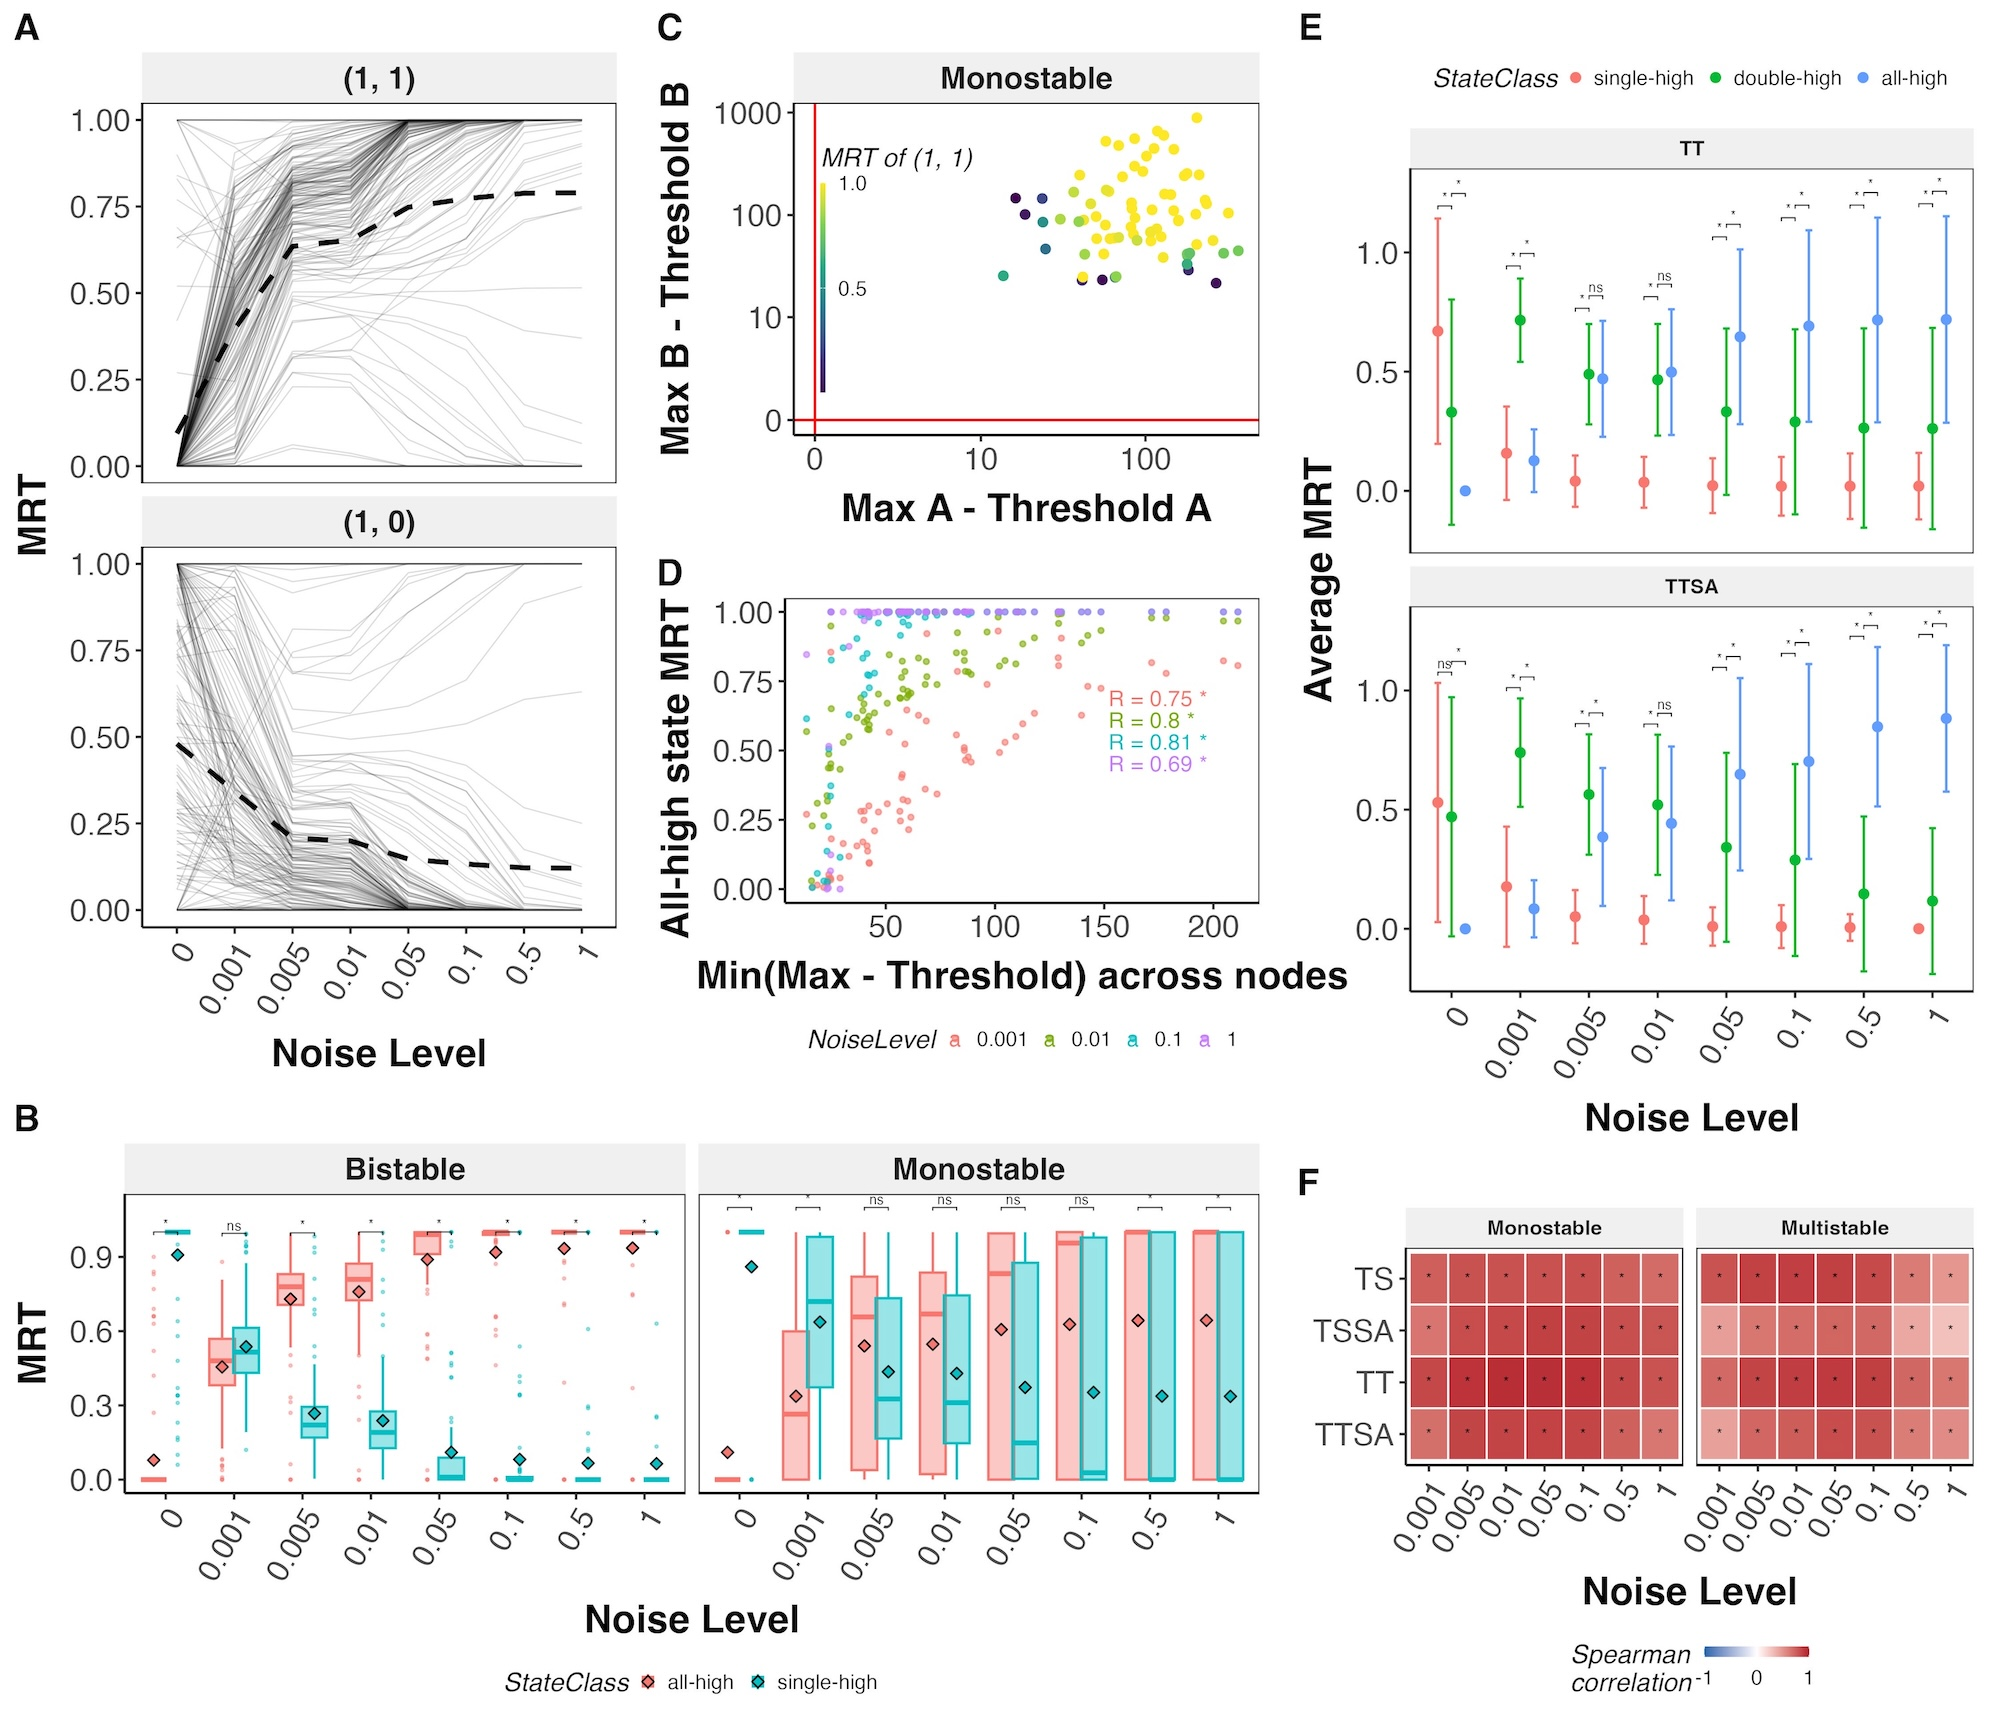
\includegraphics[width=\linewidth]{Figs/Fig3.jpg}
    \caption{\textbf{Effect of Additive noise on the phenotypic landscape of cell-fate decision networks}
    \textbf{(A)} MRT of $(1, 1)$ and $(1, 0)$ states vs.\ noise level for the TS network, individual parameter-set trajectories (gray) with population mean (dashed).
    \textbf{(B)} MRT boxplots for the TS network, monostable vs.\ bistable parameter sets, all-high vs.\ single-high states, with paired Wilcoxon significance brackets; ``*'' $p-value<0.05$, ``ns'' not significant. 
    \textbf{(C)} Reachability scatter for TS monostable parameter sets at $\sigma = 0.1$: each node's (max expression $-$ threshold) margin on the x/y axes, colored by MRT of the (1,1) state.
    \textbf{(D)} Spearman correlation between the minimum reachability margin across nodes and MRT of the (1,1) state, across four noise levels (0.001, 0.01, 0.1, 1), TS monostable parameter sets.
    \textbf{(E)} MRT vs.\ noise level for TT and TTSA, single-high $\to$ double-high $\to$ all-high state classes shown as Mean $\pm$ SD across all parameters, with paired Wilcoxon significance brackets between adjacent classes; ``*'' $p-value<0.05$, ``ns'' not significant. 
    \textbf{(F)} Heatmap of the Spearman correlation between minimum reachability margin and MRT of the all-high state, across networks (TS, TSSA, TT, TTSA), noise levels, and stability class (monostable vs.\ multistable); ``*'' $p-value<0.05$, ``ns'' not significant.
}
    \label{fig:3}
\end{figure}

\begin{figure}
    \centering
    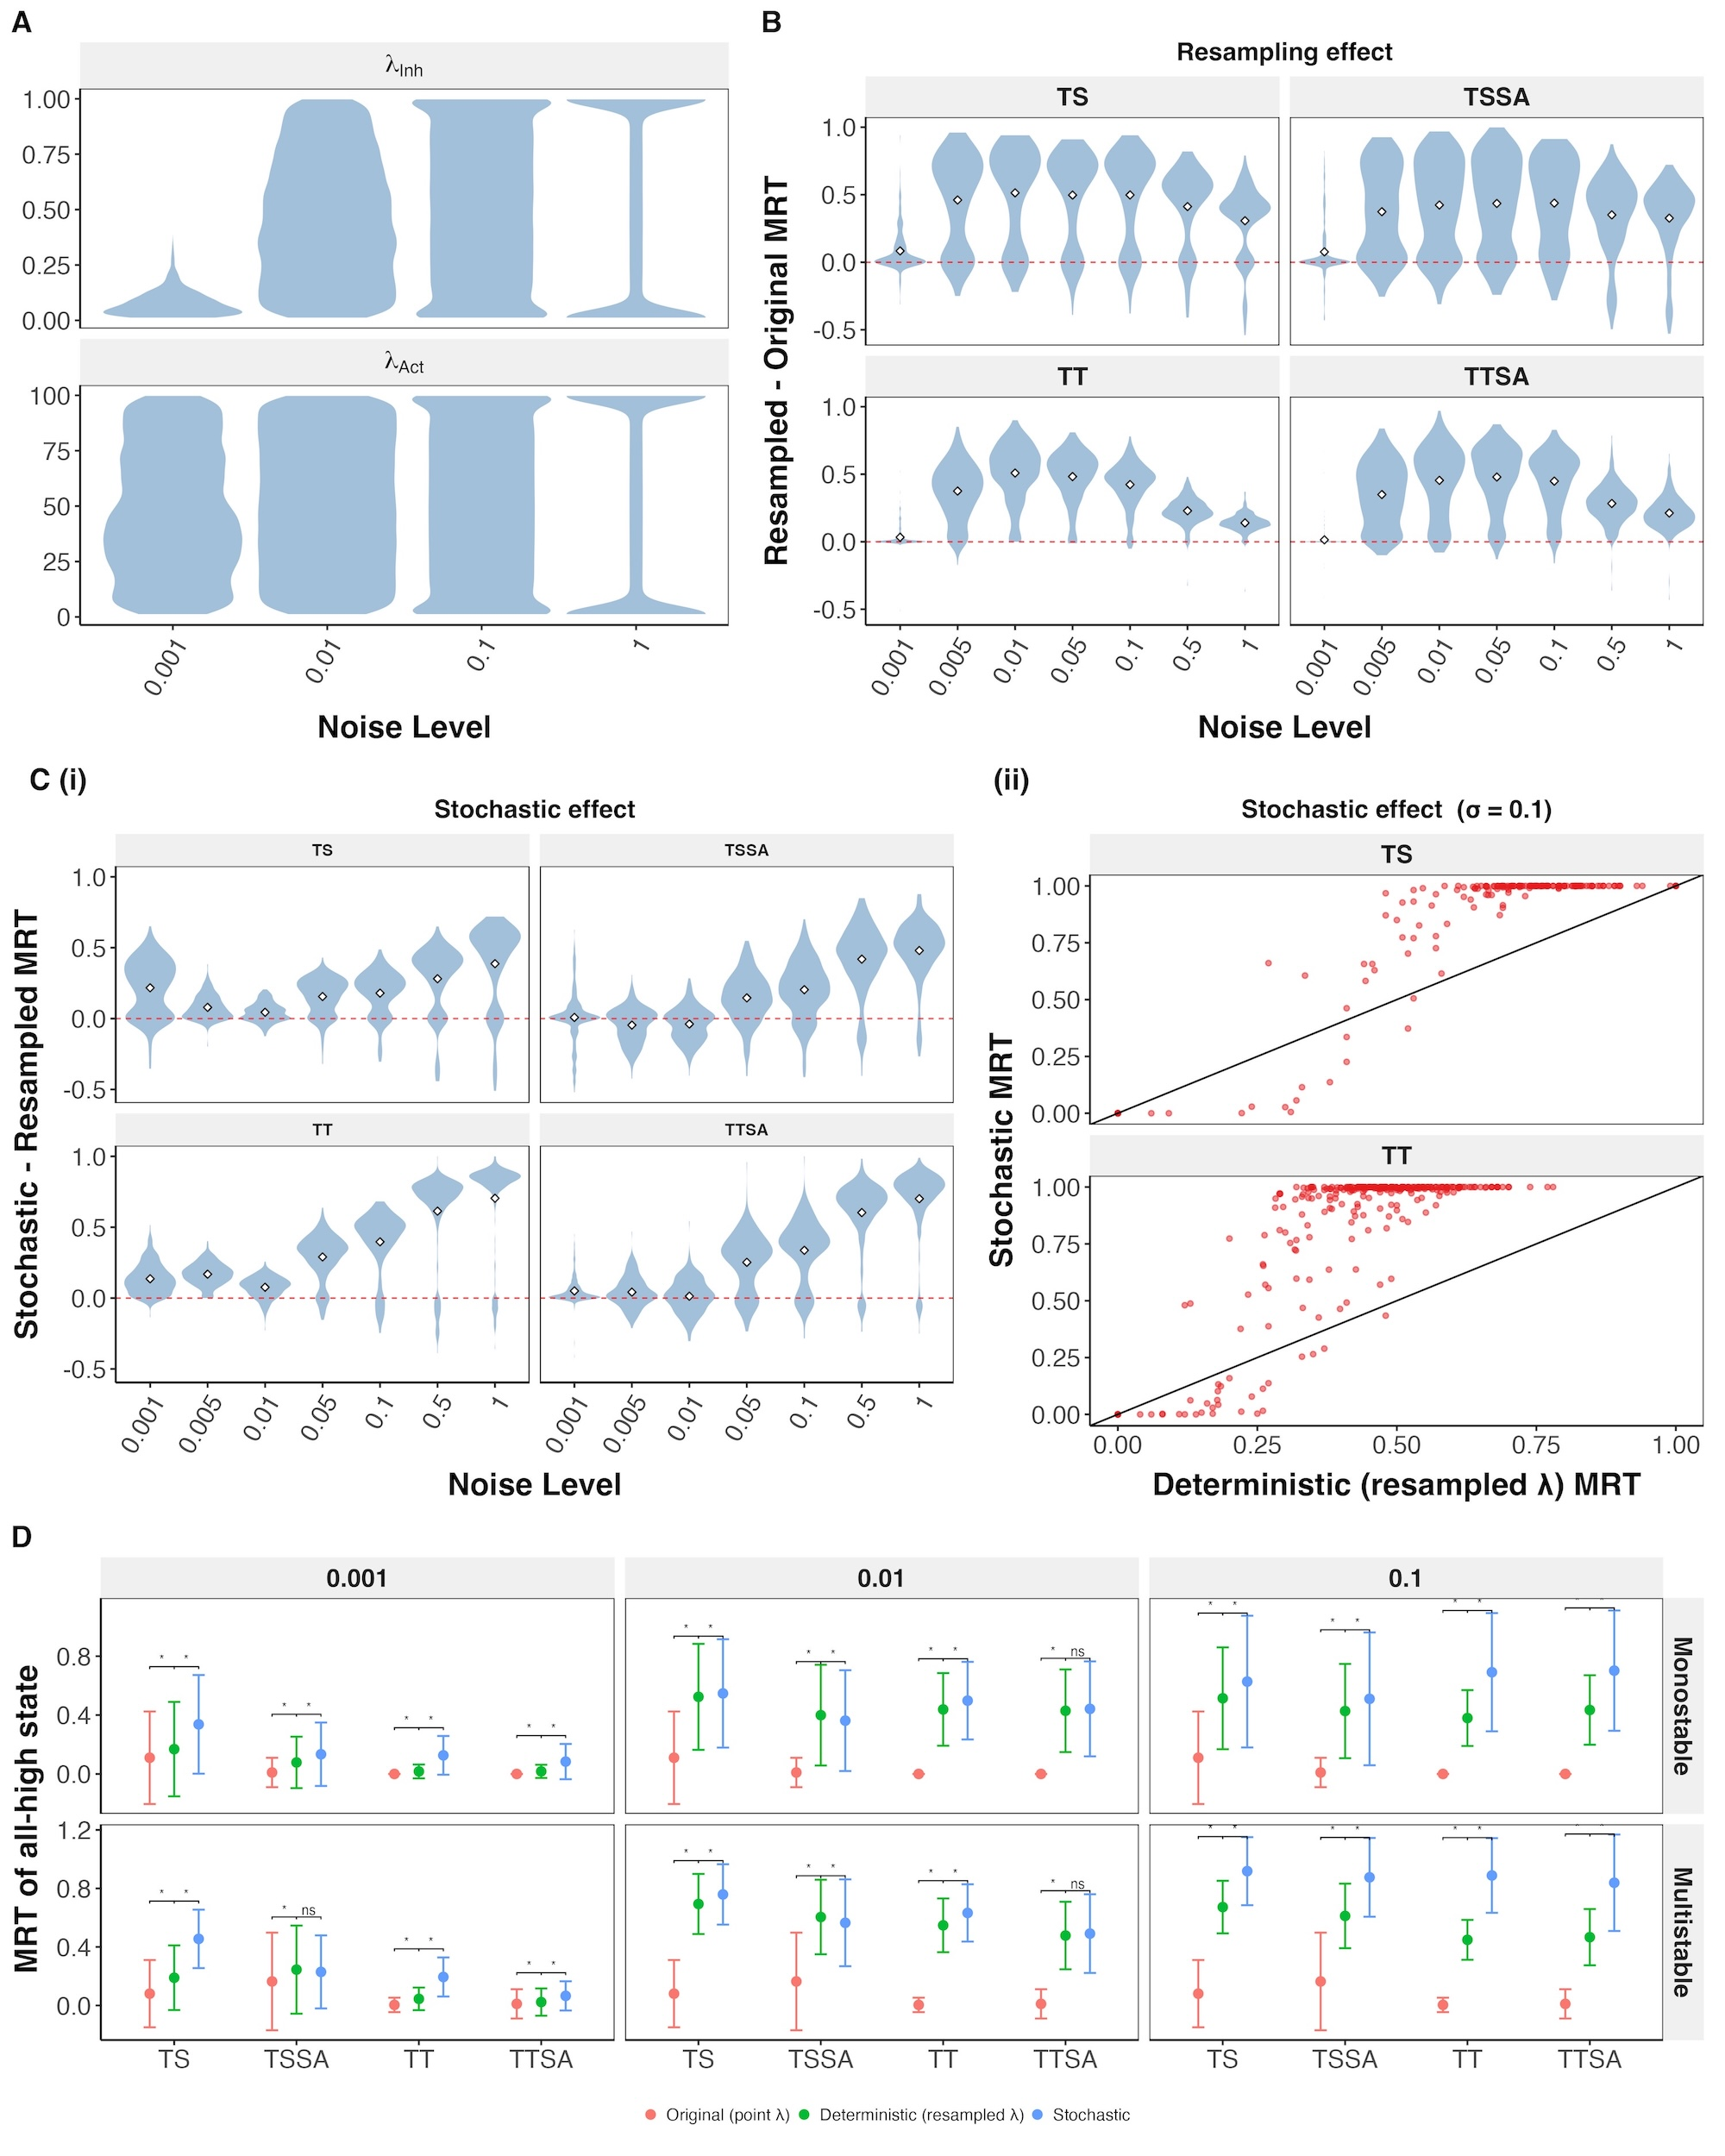
\includegraphics[width=\linewidth]{Figs/Fig4.jpg}
    \caption{\textbf{The additive noise effect combines a $\lambda$-distribution shift with an additional stochastic contribution.}
    \textbf{(A)} Distribution of $\lambda$ (Hill-function threshold) values across the parameter ensemble, for (i) inhibitory and (ii) activation-type edges, at four noise levels (Additive noise).
    \textbf{(B)} Distribution of the resampling effect - difference in deterministic MRT after $\lambda$-resampling and the original point-$\lambda$ deterministic MRT for the all-high state, shown as violin plots across all noise levels, for TS, TSSA, TT, and TTSA.
    \textbf{(C)} (i) Same as B, but for Stochastic effect (stochastic MRT minus resampled-$\lambda$ deterministic MRT). (ii) Scatter plot of resampled-$\lambda$ deterministic vs.\ stochastic MRT of the all-high state at $\sigma = 0.1$, for TS and TT, illustrating the underlying sigmoidal relationship the violin's signed difference alone does not show. Each point is a parameter set.
    \textbf{(D)} All-high-state MRT (mean $\pm$ SD over all monostable and multistable parameter sets) for TS, TSSA, TT, and TTSA, comparing the original point-$\lambda$ deterministic run, the $\lambda$-resampled deterministic run, and the full stochastic simulation; faceted by stability class of the parameter sets (rows) and noise level (columns: 0.001, 0.01, 0.1), with paired Wilcoxon significance brackets; ``*'' $p-value<0.05$, ``ns'' not significant.}
    \label{fig:3b}
\end{figure}


\begin{figure}
    \centering
    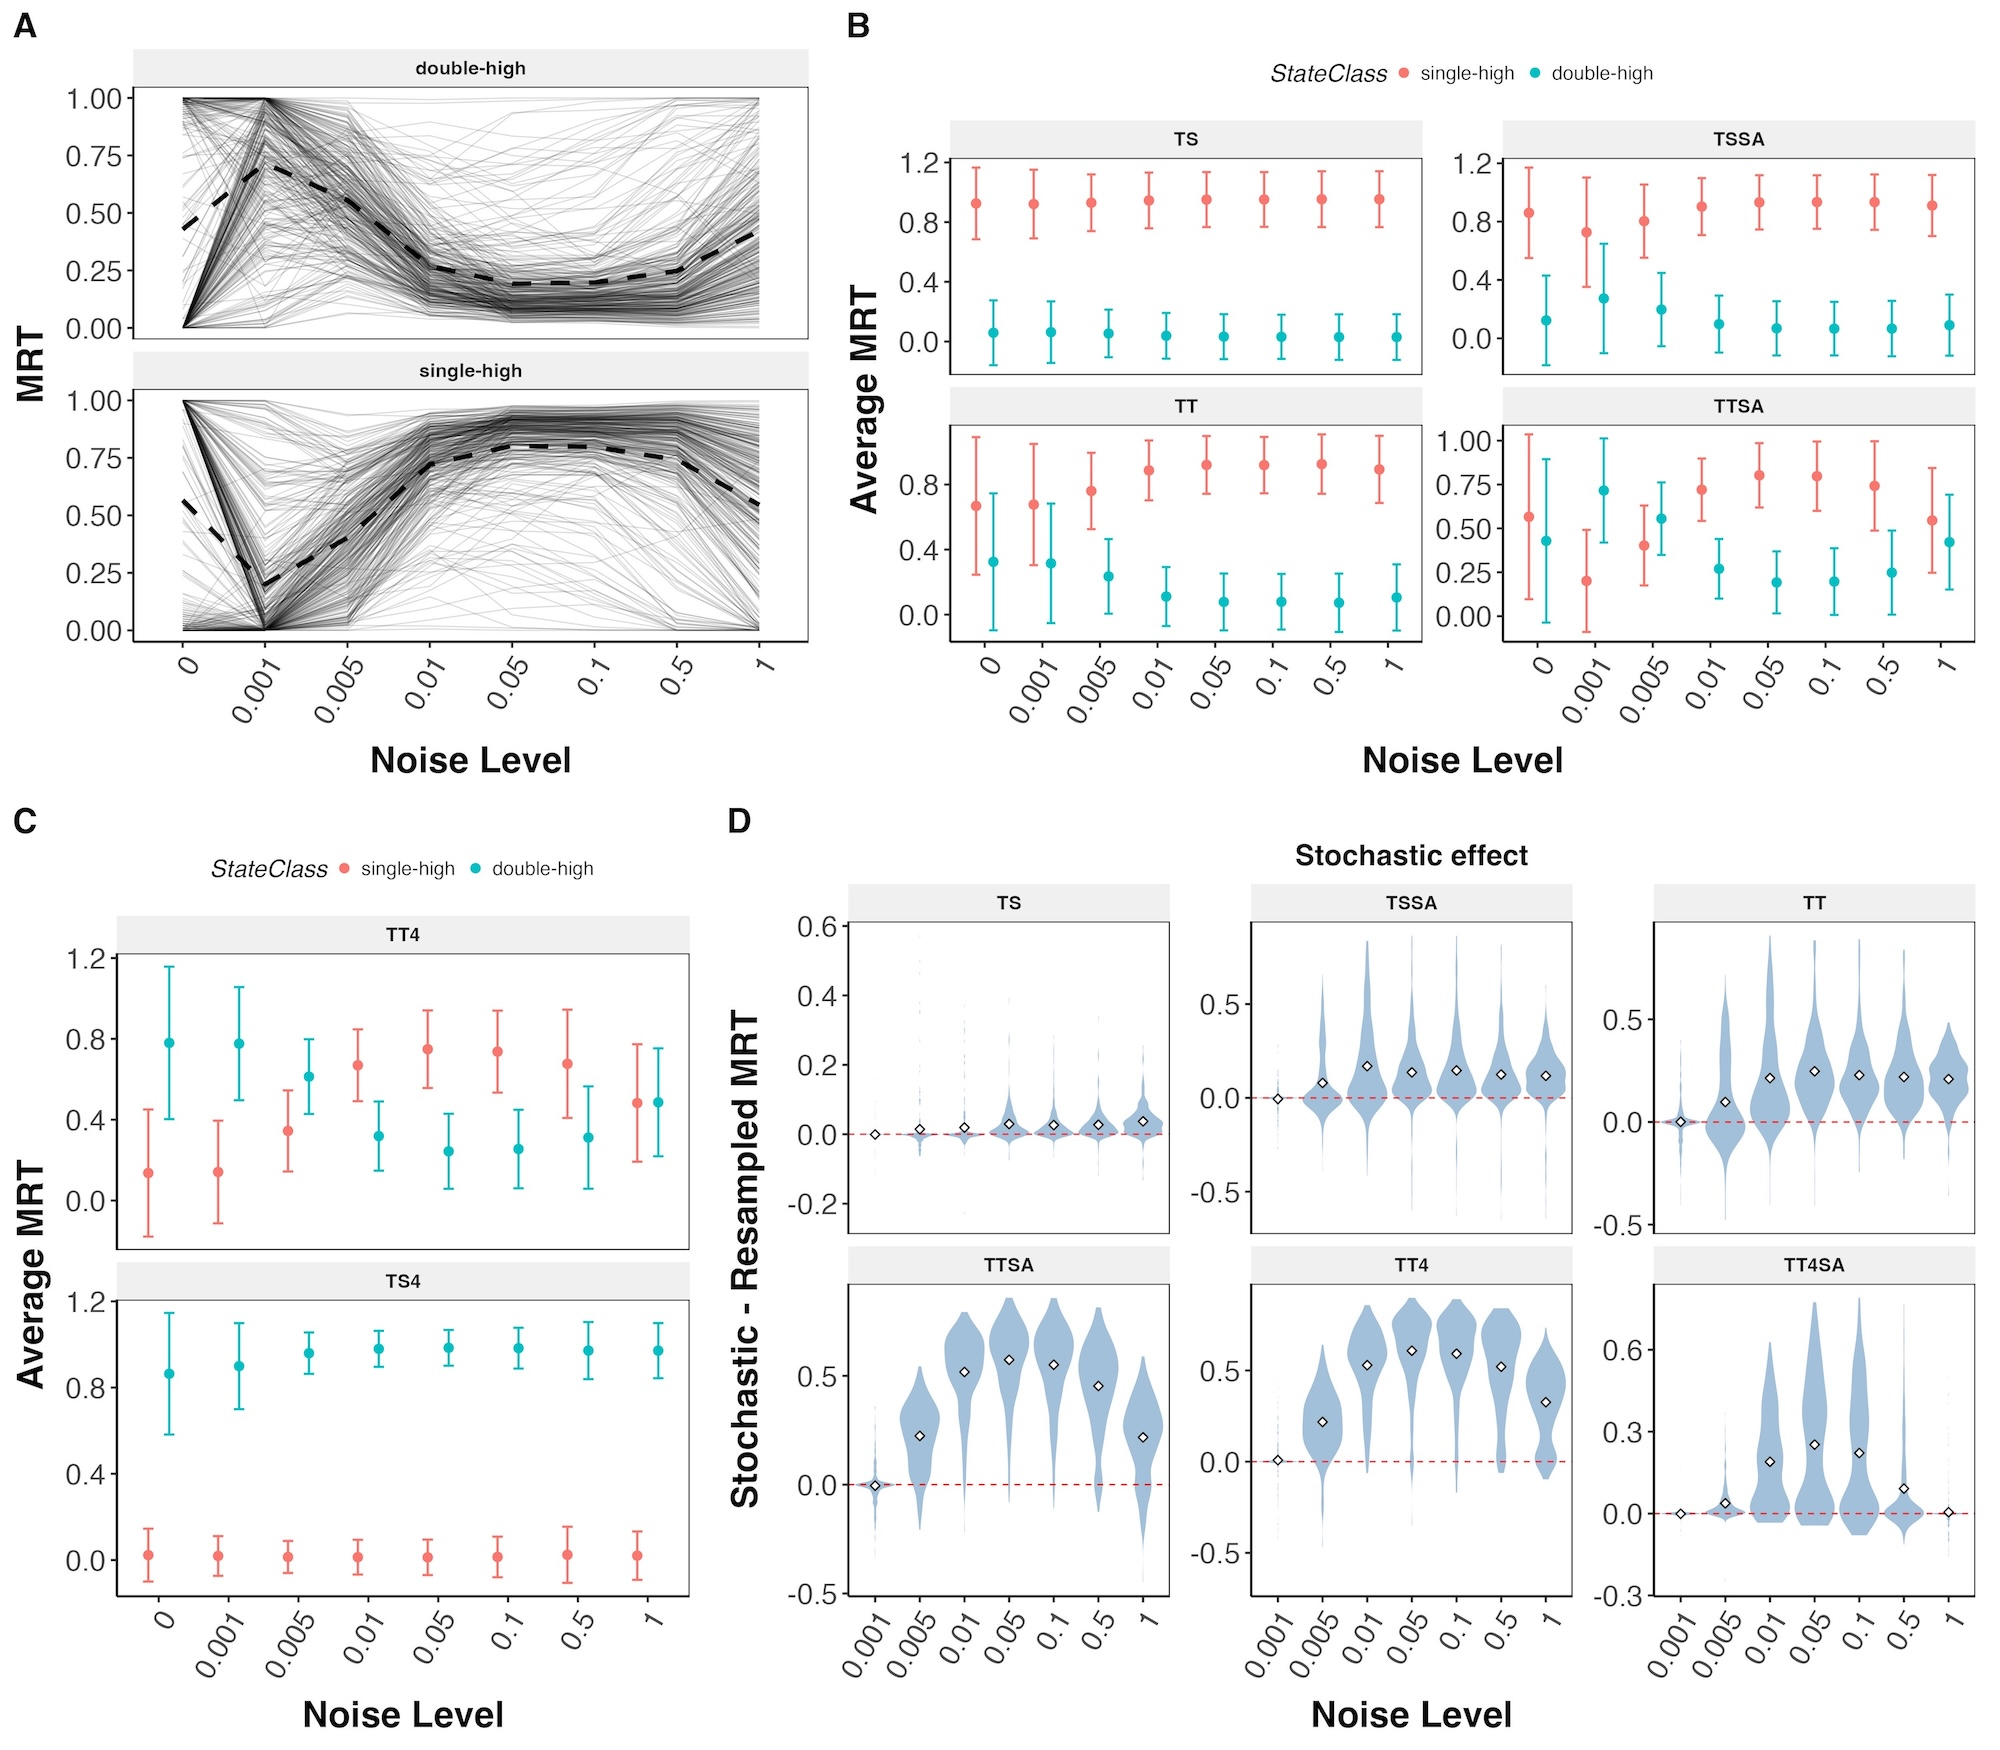
\includegraphics[width=\linewidth]{Figs/Fig5.jpg}
    \caption{Effect of multiplicative noise on the phenotypic landscape of cell-fate decision networks.
    \textbf{(A)} MRT vs.\ noise level for the TTSA network, single-high and double-high states.
    \textbf{(B)} Average MRT of single-high vs.\ double-high states vs.\ noise level, for TS, TSSA, TT, and TTSA.
    \textbf{(C)} Same, for the 4-node networks TT4 and TS4.
    \textbf{(D)} Stochastic effect (as in Fig.\ 4C(i)) for the single-high state, across noise levels, for TS, TSSA, TT, TTSA, TT4, and TT4SA.
}
    \label{fig:4}
\end{figure}

\begin{figure}
    \centering
    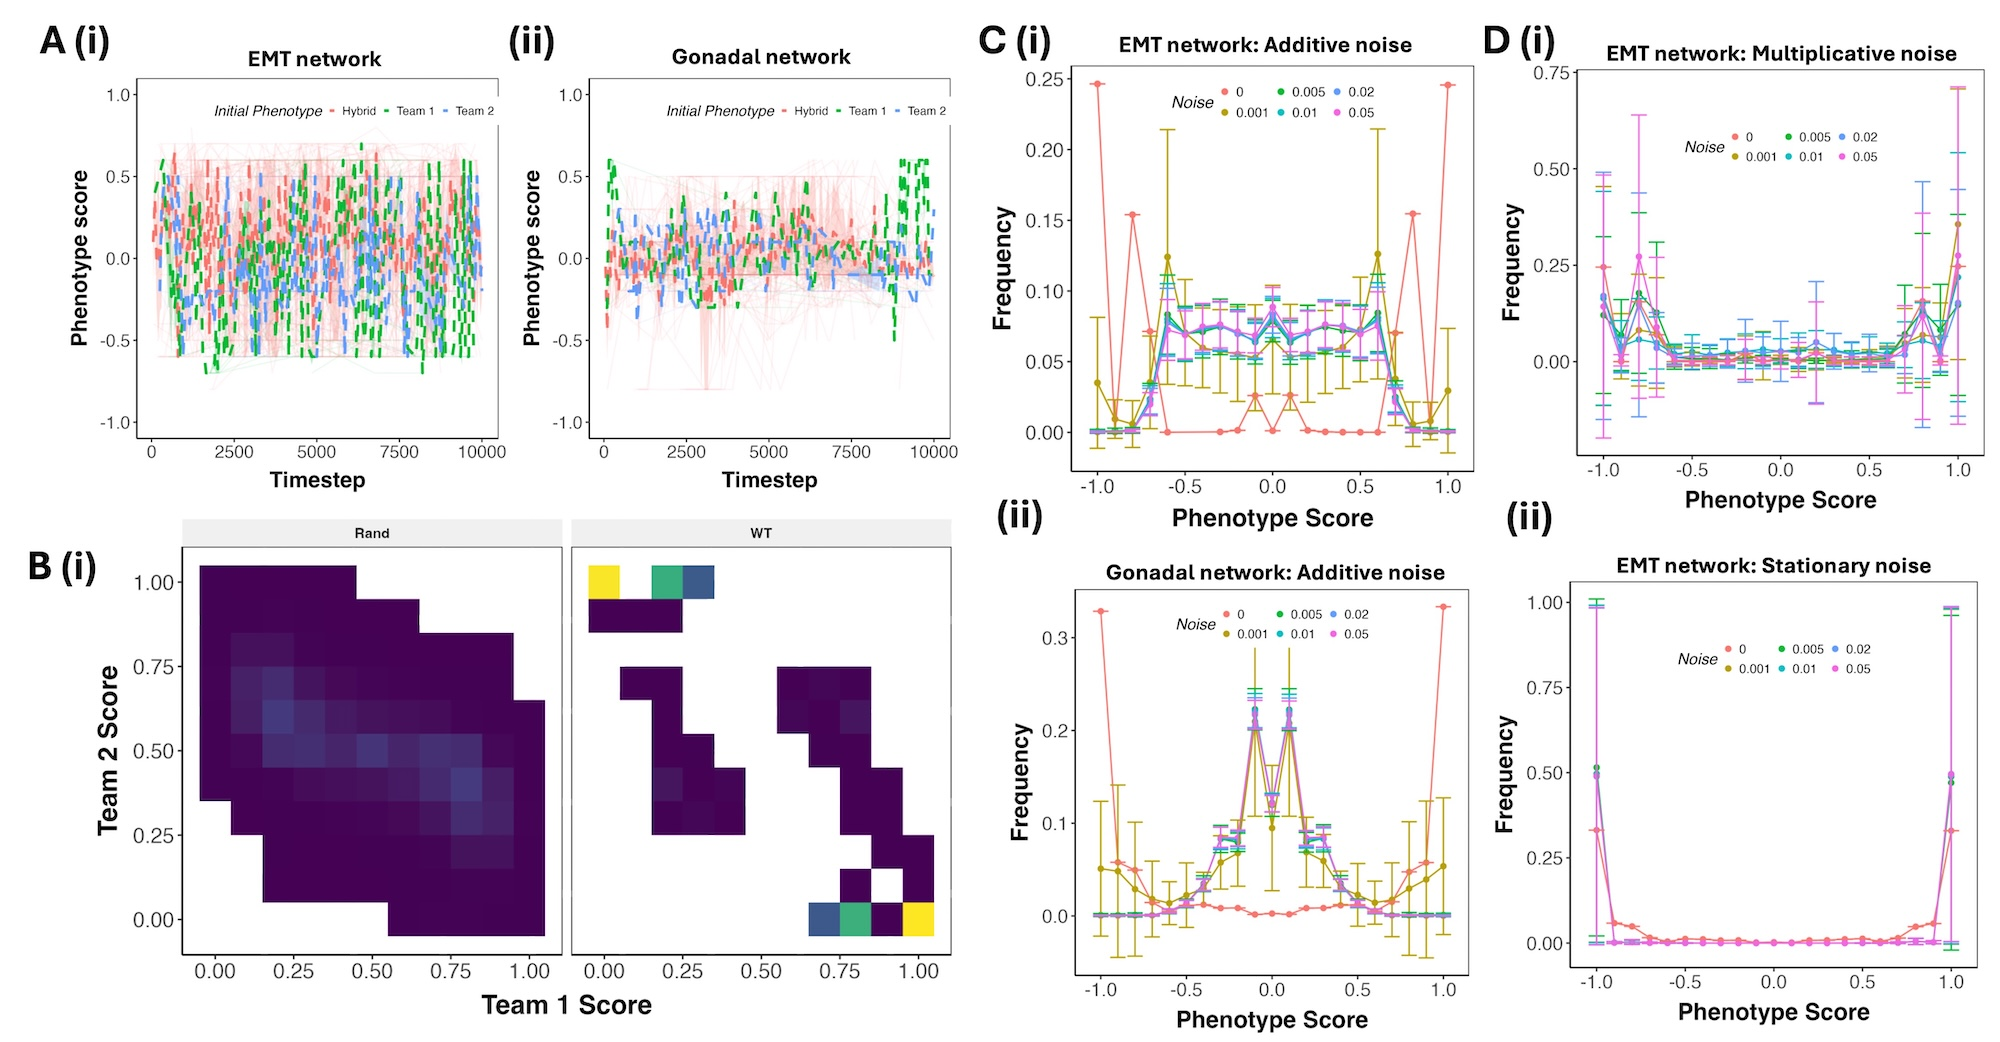
\includegraphics[width=\linewidth]{Figs/Figure4.jpg}
    \caption{\textbf{Effect of regulatory noise on large biological networks} A) Representative trajectories of the phenotypic score for EMT network (i) and Gonadal network (ii) at additive noise of 0.05 magnitude. B) Density of team scores across the representative trajectory of the EMT network, with frequency represented on a scale from low (blue) to high (yellow). WT represents the frequency of team score configurations obtained from the steady states of the unperturbed network, while Rand represents that of the simulations corresponding to the trajectories in A. C) Relative frequency (equivalent to MRT) of different phenotypic scores across 1000 simulation trajectories of additive noise over simulation time for (i) EMT network, (ii) Gonadal network. D) Same as C, but for Multiplicative and Stationary noise for EMT network.}
    \label{fig:5}
\end{figure}


\begin{figure}
    \centering
    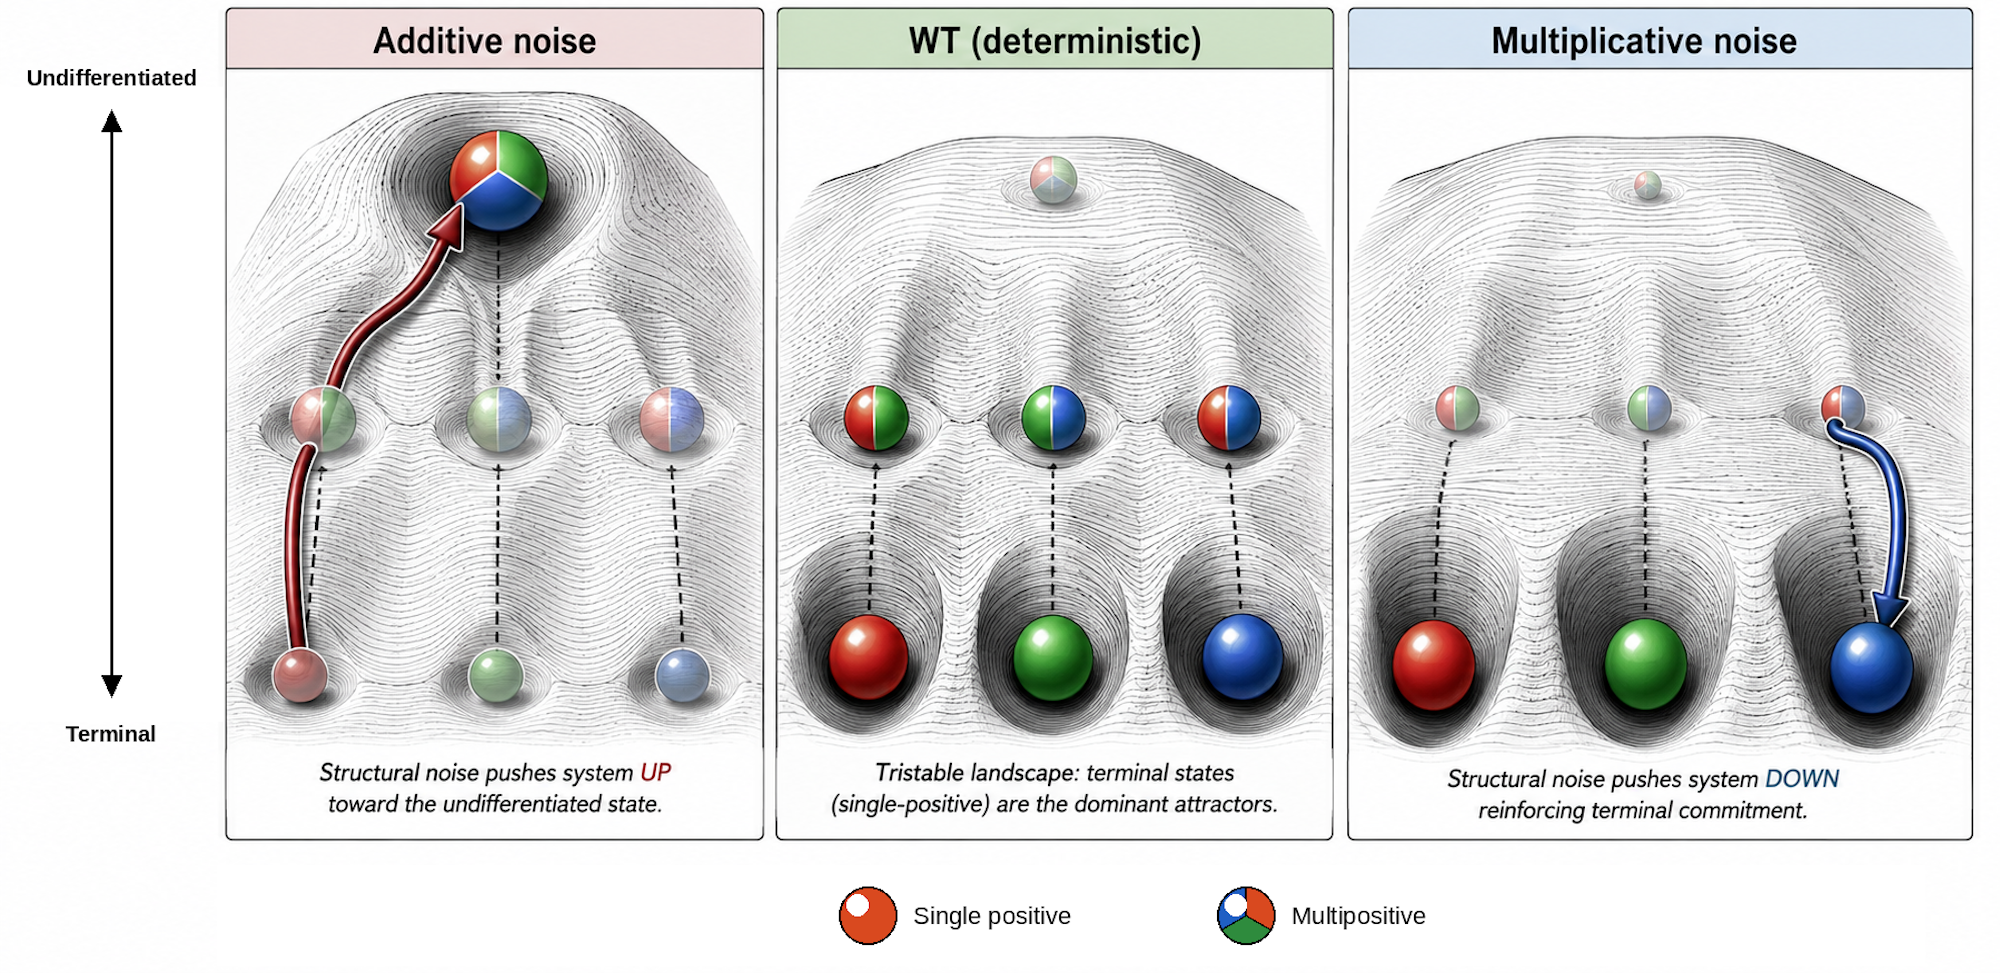
\includegraphics[width=\linewidth]{Figs/Schematic.png}
    \caption{\textbf{Graphical representation of the effect of regulatory noise on the cell-fate decision landscape supported by GRNs}}
    \label{fig:schematic}
\end{figure}
\newpage
\beginsupplement

\section{Supplementary Figures}

\begin{figure}[!ht]
    \centering
    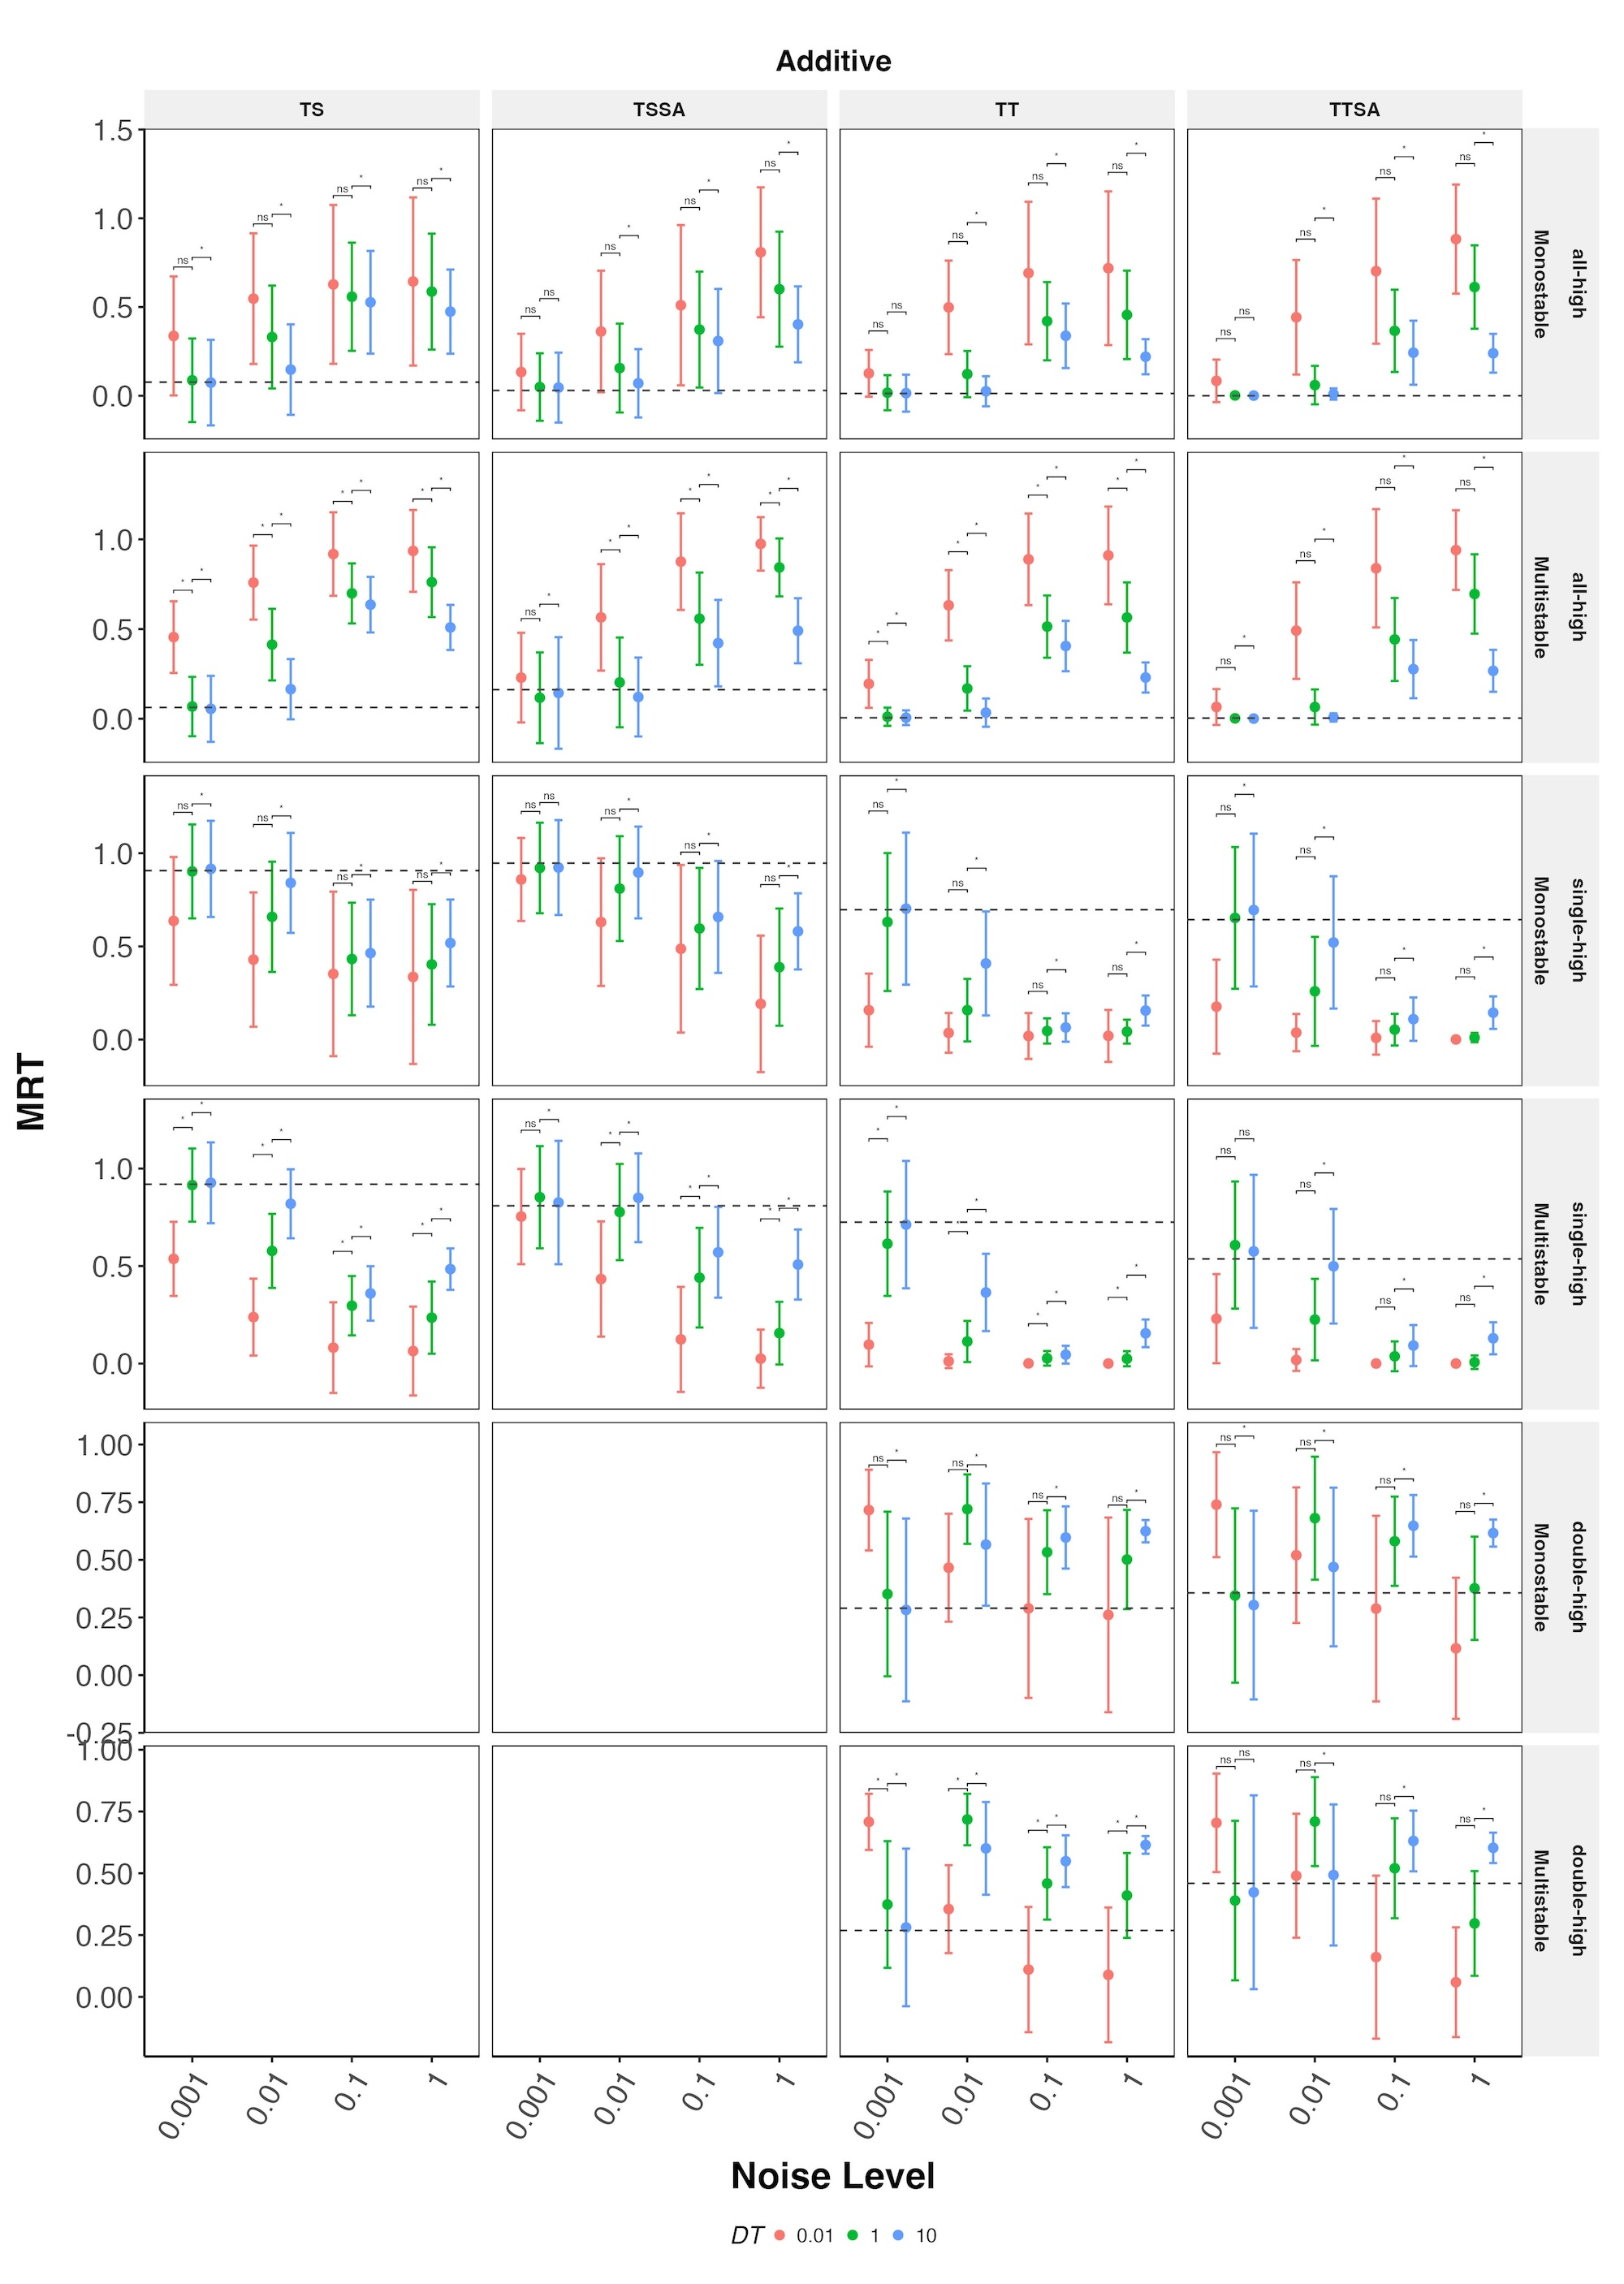
\includegraphics[width=0.8\linewidth]{Figs/Fig4S3.jpg}
    \caption{Comparison of MRTs for additive noise simulated at different values of $dt$}
    \label{fig:3bS3}
\end{figure}

\begin{figure}
    \centering
    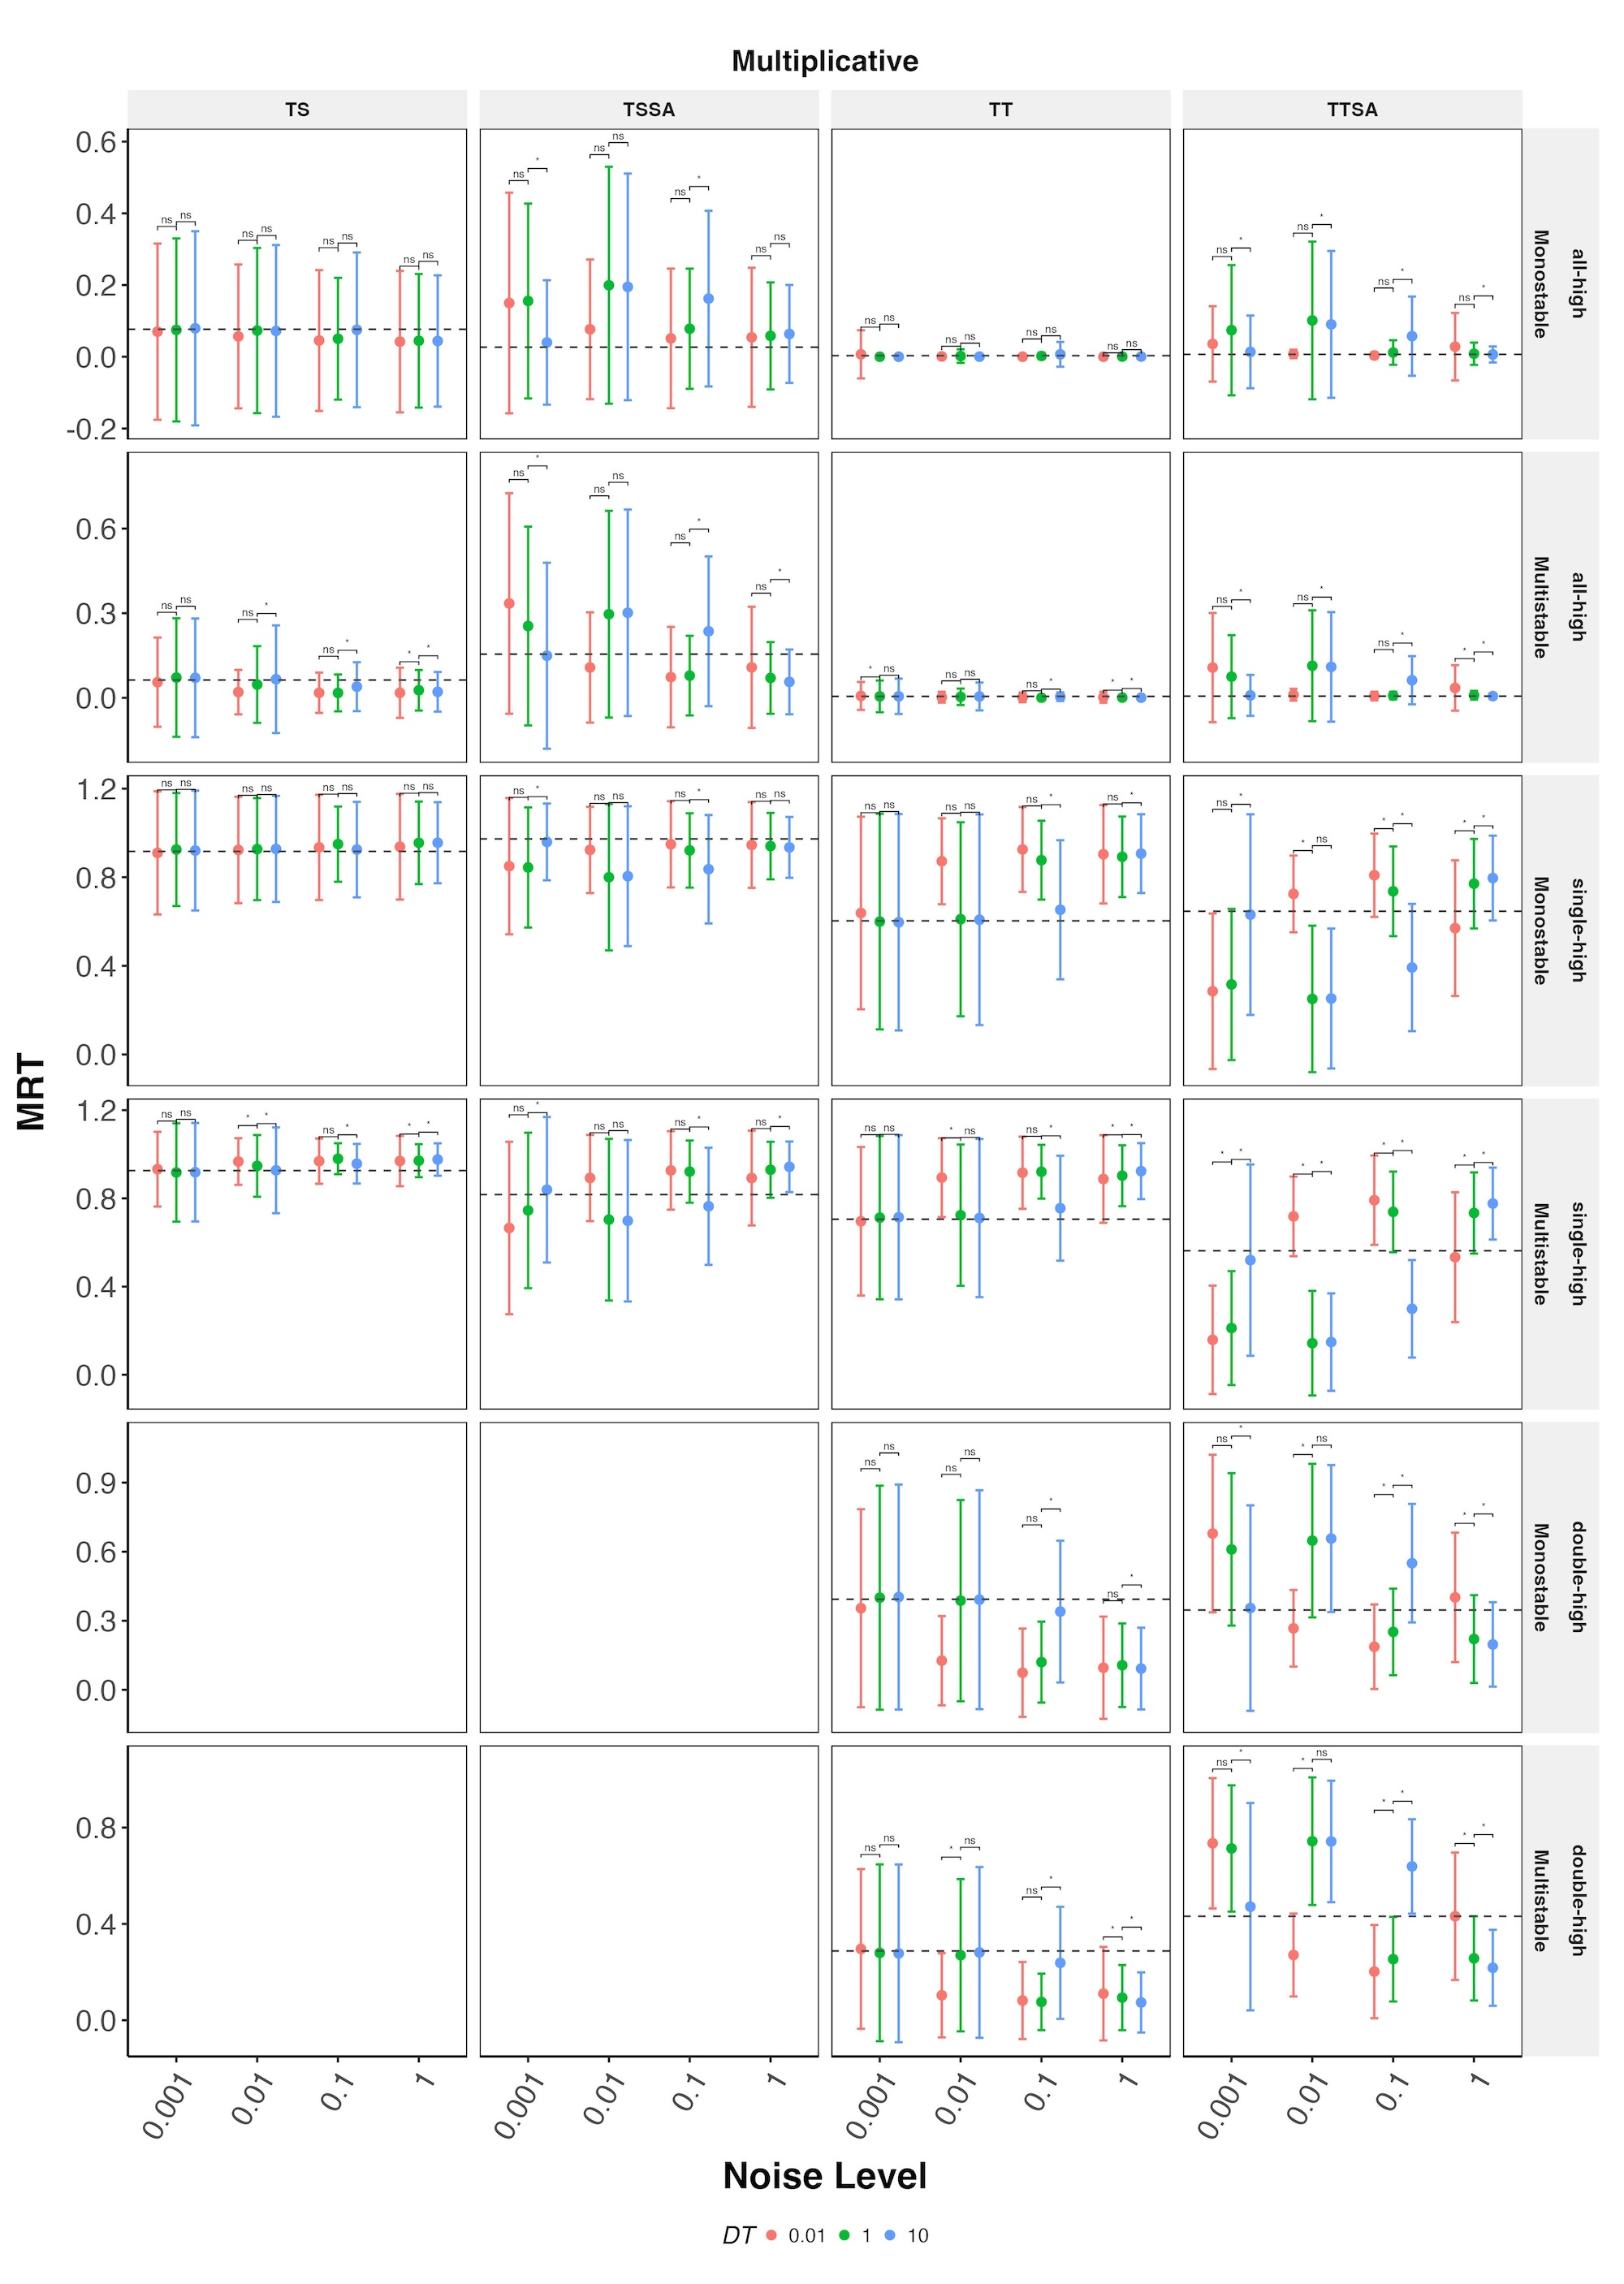
\includegraphics[width=0.8\linewidth]{Figs/Fig5S3.jpg}
    \caption{Comparison of MRTs for multiplicative noise simulated at different values of $dt$}
    \label{fig:4S3}
\end{figure}

\end{document}
